% !TEX root = manuscrit.tex

\part[Verification of mobile robot protocols]{Verification of mobile robot protocols: the exploration case}
\label{part:verif}      

%%%%%%%%%%%%%%%%%%%%%%%%%%%%%%%%%%%%%%%%%%%%%%%%%%
%%%%%%%%%%%%%%%%%%%%%Exploration%%%%%%%%%%%%%%%%%%%%%%%%
%%%%%%%%%%%%%%%%%%%%%%%%%%%%%%%%%%%%%%%%%%%%%%%%%%


                                                                               
%%%%%%%%%%%%%%%%%%%%%%%%%%%%%%%%%%%%%%%%%%%%%%%%%%%%
%%%%%%%%%%%%%%%%%%%%%%    FLO    %%%%%%%%%%%%%%%%%%%%%%%%%
%%%%%%%%%%%%%%%%%%%%%%%%%%%%%%%%%%%%%%%%%%%%%%%%%%%%
	\chapter{Flocchini Algorithm}
The problem of exploration with stop on a ring was first defined in~\cite{flocchini_computing_2007}.
It is proved there that the problem cannot be solved by a deterministic algorithm when the
number $k$ of robots and the ring size $n$ are not corpime.   
  
We consider the algorithm from Flocchini \emph{et al.} that solves the problem for $k \geq 17$, 
with $k$ and $n$ coprime.
The original paper only contains an informal description of the
algorithm, Thus, our first contribution is to formally express the
algorithm in order to remove ambiguities.  
We end by the verification results.  
	\label{sec:flo}
	
	
\section{Specification of exploration with stop} 
\label{subsub: specification}
For any ring and any
initial configuration where no two robots are located on the same vertex, 
a protocol solves the problem of exploration with stop if within
finite time, it
guarantees the following two properties: 
\begin{itemize}
\item[\emph{(i)}] \emph{Exploration}: 
 Each node of the ring is visited by at least one robot, and
\item[\emph{(ii)}] \emph{Termination}:  Eventually, the robots reach a
  configuration where they all remain idle (their $\textit{LC}_i$
  action leads to $r_i.\Idle$).
\end{itemize}
Note that this last property requires robots to ``remember'' how much
of the ring has been explored \emph{i.e.}, these oblivious robots
must be able to distinguish between various stages of the exploration
process simply by their current view.
%One key tool to
%identify
%configuration is the ``tower'' (a node where more than one robot are
%simultaneously present) that are forbidden in any initial configuration.

These two properties can be expressed in \textsf{LTL} (see Section~\ref{def:LTL}) as follows: 
\begin{itemize}%[parsep=0cm, itemsep=0cm, topsep=0cm] 
\item \emph{Exploration}: 
$\bigwedge\limits_{i=1}^n\F\bigvee\limits_{j=1}^k\big(c(r_j)=i\big)$. 
\item \emph{Termination}: 
$\bigwedge\limits_{j=1}^k\F\G\big(\neg r_j.\Front 
\wedge \neg r_j.\Back)$.
\end{itemize}

\begin{definition} A protocol solves the problem of ring exploration
  with stop if from any initial configuration, the following formula
  holds: 
  $$\textit{Fairness} \ \Rightarrow \ (\textit{Exploration} \ \wedge 
\ \textit{Termination})$$
\end{definition}


	
	
	
		\section{Formalisation of the algorithm}
In this algorithm~\cite{flocchini_computing_2007}, a set of $k$ identical robots explore an unoriented
ring of $n$ anonymous (\emph{i.e.}, identical) nodes, with $n>0$ and
$k>0$.  Initially there is no tower, thus $k
\leq n$. Since the case where $n=k$ is trivial, we assume from now on
that $k<n$. Moreover, $n$ and $k$ are assumed to be co-prime. The algorithm is
divided into three phases, the \emph{Set-Up} phase, the
\emph{Tower-Creation} phase and the \emph{Exploration} phase. In the
Set-Up phase, all robots are gathered in one group or two groups of
the same size.  In the second phase, the goal is to create one or two
towers per block according to the parity of the blocks. The last phase
is the exploration of the ring.

In order to express the algorithm as a decision function 
(and then in a guarded action language), some
definitions and notations are introduced, related to a given
configuration, and examples from the rings of Figure~\ref{fig:floDef} are
given along these definitions.
\begin{figure}[htbp] 
\begin{center} 
\subfloat[]{
\centering
%\includegraphics[scale=0.9]{figex1}
\begin{tikzpicture}[scale=0.7, transform shape, thick] 
\node[circle, minimum size =8.25em, draw, thick] (C0){};

\foreach \i in {0, ..., 16}
\node[circle, minimum size =1em, draw, fill=white, thick]at(\i*21: 1.7) (\i){};

 
\node[circle, minimum size =1em, fill=black]at(0: 1.7) (0){};
\node[circle, minimum size =1em, fill=black]at(1*21: 1.7) (1){};
\node[]at(1*25: 2.2) (1+){\Large$r_3$};
\node[circle, minimum size =1em, fill=black]at(4*21: 1.7) (4){};
\node[]at(4*21: 2.2) (4+){\Large$r_2$};
\node[circle, minimum size =1em, fill=black]at(7*21: 1.7) (7){};
\node[]at(7*21: 2.2) (7+){\Large$r_1$};
\node[circle, minimum size =1em, fill=black]at(9*21: 1.7) (9){};
\node[circle, minimum size =1em, fill=black]at(10*21: 1.7) (10){};
\node[circle, minimum size =1em, fill=black]at(11*21: 1.7) (11){};
\node[circle, minimum size =1em, fill=black]at(14*21: 1.7) (14){};
\node[circle, minimum size =1em, fill=black]at(15*21: 1.7) (15){};
\node[circle, minimum size =1em, fill=black]at(16*21: 1.7) (16){};
%b1
\node[left = 0.1em of 9](lu){};
\node[left = -0.3em of 11](lb){};
\node[left = 0.1em of lu](llu){};
\node[left = 2.05em of lb](llb){};
\draw[thin] (lu.center)--(llu.center)--(llb.center)--(lb.center);
\node[left = 1.8em of 10](b1){\Large$b1$};
%b2
\node[right = 0.1em of 1](ru){};
\node[right = -0.6em of 14](rb){};
\node[right = 0.1em of ru](rru){};
\node[right = 3.1em of rb](rrb){};
\draw[thin] (ru.center)--(rru.center)--(rrb.center)--(rb.center);
\node[right = 1.35em of 16](b2){\Large$b2$};

\end{tikzpicture}
\label{fig:def1} 
}
\subfloat[]{
\centering
%\includegraphics[scale=0.9]{figex2}
\begin{tikzpicture}[node distance =15em, scale=0.7, transform shape, thick] 
\node[circle, minimum size =8.25em, draw, thick] (C0){};

\foreach \i in {0, ..., 16}
\node[circle, minimum size =1em, draw, fill=white, thick]at(\i*21: 1.7) (\i){};
 
\node[circle, minimum size =1em, fill=black]at(1*21: 1.7) (1){};
\node[]at(1*25: 2.2) (1+){\Large$r_3$};
\node[circle, minimum size =1em, fill=black]at(4*21: 1.7) (4){};
\node[]at(4*21: 2.2) (4+){\Large$r_2$};
\node[circle, minimum size =1em, fill=black]at(7*21: 1.7) (7){};
\node[]at(7*21: 2.2) (7+){\Large$r_1$};
\node[circle, minimum size =1em, fill=black]at(9*21: 1.7) (9){};
\node[circle, minimum size =1em, fill=black]at(11*21: 1.7) (11){};
\node[circle, minimum size =1em, fill=black]at(14*21: 1.7) (14){};
\node[circle, minimum size =1em, fill=black]at(16*21: 1.7) (16){};

%b1
\node[left = 0.1em of 7](lu){};
\node[left = -0.25em of 11](lb){};
\node[left = 0.25em of lu](llu){};
\node[left = 1.5em of lb](llb){};
\draw[thin] (lu.center)--(llu.center)--(llb.center)--(lb.center);
\node[left = 0.8em of 9](b1){\Large$b1$};
%b2
\node[right = 0.1em of 1](ru){};
\node[right = -0.6em of 14](rb){};
\node[right = 0.1em of ru](rru){};
\node[right = 3.1em of rb](rrb){};
\draw[thin] (ru.center)--(rru.center)--(rrb.center)--(rb.center);
\node[right = 1.35em of 16](b2){\Large$b2$};


\end{tikzpicture} 
\label{fig:def2} 
}
\caption{Illustration of the definitions.} 
\label{fig:floDef} 
\end{center} 
\end{figure} 

\begin{itemize}%[parsep=0cm, itemsep=0cm, topsep=0cm] 
\item The \emph{interdistance} $d$ is the minimum distance between all
  pairs of distinct robots in the configuration, where distance is
  counted in number of edges. Hence, an interdistance $d=0$
  corresponds to the presence of (at least) two robots on a same node.

  For the configuration a of Figure~\ref{fig:floDef}, the interdistance
  is $1$, while it is $2$ for b.  

\item A \emph{block} is a maximal set of at least 2 robots that are
  located every $d$ nodes (where $d$ is the interdistance of the
  configuration). Maximality means that (at least) the $d$ adjacent
  nodes of a block in both directions are free.  Note that a block
  contains at most $d-1$ consecutive free nodes.
  We denote by $\textit{Blocks}$ the set of blocks.
\item The \emph{size} of a block $b$, denoted by $b.\textit{size}$, is
  the number of robots in this block.

  In configuration a, there are two blocks of size $3$ and $5$, 
  while there are two blocks of size $3$ in b.

\item $\textit{Between}(b_1, b_2)$ is a pair of natural numbers
  counting the number of blocks between two blocks $b_1$ and $b_2$
  (one integer for each direction).  In both a and b, 
  $\textit{Between}(b1, b2)$ is equal to $(0, 0)$.
   
\end{itemize}
We also define the following predicates: 
\begin{description}%[parsep=0cm, itemsep=0cm, topsep=0cm]
\item [$\textrm{Isolated}(r)$: ] this predicate is true if $r$ is an
  isolated robot. A robot is \emph{isolated} if it is not part of
  a block, that is, if in both directions its $d$ adjacent nodes are
  free.

  In (a), $\textrm{Isolated}(r_1) = \true$, 
  $\textrm{Isolated}(r_2)=\true$ and in (b), 
  $\textrm{Isolated}(r_2)=\true$.

\item [$\textrm{Border}(r, b)$: ] this predicate is true if robot $r$ is
  a border of the block $b$. A robot $r$ is a \emph{border} of a block
  if it is one of the extremal robot that forms this block.
  
  For example $\textrm{Border}(r_1, b1)$ is false in a and true in b.
\item [$\textrm{Neighbor}(x, y)$: ] this predicate is true if $x$ and
  $y$ are neighbors, $x$ and $y$ being either robots or blocks. Two
  robots, two blocks or a robot and a block are \emph{neighbors} if
  there exists at least one direction such that only free nodes exist
  between them.
  
  $\textrm{Neighbor}(r_1, r_2)$ and $\textrm{Neighbor}(r_2, b2)$ are
  true in both (a) and (b), but the predicate $\textrm{Neighbor}(r_2, b1)$ is false
  in a and true in b.
\item [$\textrm{Leading}(x)$: ] this predicate is true if $x$ is a
  leading block or a leading robot. A robot is leading if its view is
  minimal (among the different $\view^{\min\_r}$). Such a robot is
  called a \emph{leader}. A block $b$ is \emph{leading} if it has a
  border robot which is a leader.

  In the example of Figuren\ref{fig:floDef}, only $\textrm{Leading}(r_3)$ is true, Hence, also
  $\textrm{Leading}(b2)$, while in (b), both $\textrm{Leading}(r_1)$
  and $\textrm{Leading}(r_3)$ are true.
 \end{description}
Finally, the distance $\textit{dist}(x, y)$ between two neighbors $x$
 and $y$ in $\textit{Blocks} \cup \textit{Rob}$ is the minimum length
 of a path between them containing only free nodes.

 We now formally describe each phase of the algorithm as
 performed by each robot.
 
 \subsection{The Set-Up Phase}\label{setup} 
 The aim of this phase is to gather robots on particular
 configurations called the \emph{Set-Up final configurations}, defined
 by: $d=1$, there are no isolated robots, and each block is a leading
 block. In such a case, either all robots are in
 the same block or the robots are divided into two blocks of the same
 size, since otherwise $k$ and $n$ are not coprime anymore.

 Starting from a tower-free configuration, absence of tower will be
 maintained throughout the Set-Up phase. This is expressed by the 
 predicate:  $$\textrm{Set-Up}: = \ d > 0.$$  

 There are four types of configurations, namely $A$, $B$, $C$, $D$, 
 that form a partition of all possible tower-free
 configurations. Configurations of type $A$ contain isolated robots
 and configurations of type $B$, $C$ or $D$ contain only blocks of
 robots. Configurations of type $D$ are the Set-Up final
 configurations, configurations of type $C$ are similar(there are no 
 isolated robots, and each block is a leading block) to these
 configurations but with an interdistance $d \geq 2$. All the 
 remaining configurations without isolated robot are
 configurations of type $B$.

 For each of these configuration types, we introduce some notations, 
 sets and predicates to define the protocols executed by the robots.

\paragraph{Configurations of Type $A$.}
\label{conf-A-FLO}
In these configurations with at least one isolated robot, the protocol
is as follows: an isolated robot that is the nearest to the biggest
blocks adjacent to any isolated robot, moves toward these biggest
blocks (with $\?$ in case of equality).

These movements are made in order to remove isolated robots by
increasing the size of their biggest and nearest neighbor blocks.
Hence, after a finite number of transitions, the configuration must be
of type $B$, $C$ or $D$, with the same interdistance (recall that the
interdistance is denoted by $d$) as the starting
configuration of type $A$.\\
We define: \\
$S= \max \{b.\textit{size} \mid  b \in Blocks
  \text{ s.t. } \exists r \in \textit{Rob}: \textrm{Neighbor}(r, b) \wedge \textrm{Isolated}(r)\}$

$\text{Move}(r, b) = \left\{ \begin{array}{l l}
    r.\?  & \text{if } \view^{\max\_r} = \view^{\min\_r} \\
    r.\Back &\text{if } \view^{\max\_r} \neq \view^{\min\_r} 
\text{ and}\\
& \textit{dist}(r, b)> n - \textit{dist}(r, b)- (b.\textit{size} -1)\times d \\
   r.\Front &  \text{otherwise}
  \end{array} \right.$ \\
We also need the following predicates and sets: \\
$\begin{array}{l}\text{Type}A: = \text{Set-Up} \wedge \exists r \in \textit{Rob}: 
\textrm{Isolated}(r) \\ \end{array}$ \\
$\begin{array}{l l} \text{NearS}(r, b): = & \textrm{Isolated}(r) \wedge 
\textrm{Neighbor}(r, b) \wedge b.\textit{size} = S\\ \end{array}$ \\
$ \begin{array}{l l}\text{Closest}=&\{(r, b) \in 
\textit{Rob}\times \textit{Blocks} \mid  \text{NearS}(r, b)  \land \ 
\forall (r', b') \in \textit{Rob}\times \textit{Blocks}: \\ 
& \text{NearS}(r', b') \Rightarrow \textit{dist}(r, b) \leq \textit{dist}(r', b')
\} \end{array}$\\ 
The guarded action in type A for a robot $r$ is thus: 
$$[\text{Type}A \wedge (r, b) \in \text{Closest}]
\rightarrow \text{Move}(r, b).$$


\begin{example}
  This action is illustrated in Figure~\ref{figFloA}, where the
  isolated robot $r$ is at distance $9$ of $b_1$ (which is of maximal
  size) and $3$ of $b_2$. Since the two views of $r$ are different and
  $\textit{dist}(r, b_1)> n - \textit{dist}(r, b_1) - (b_1.\textit{size} -1)\times d$
  holds with $n=21$ and $d=2$, its move must be $r.\Back$, in the 
  opposite direction to its minimal view, as indicated by the arrow on 
  Figure~\ref{figFloA}.

\begin{figure}[htbp]
\centering 
%\includegraphics[scale=1.4]{figFloA}
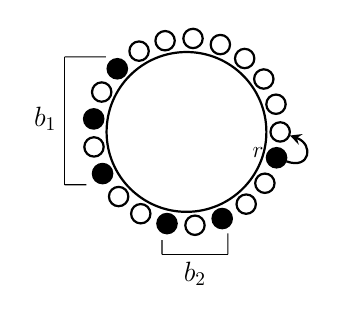
\begin{tikzpicture}[node distance =15em, scale=0.7, transform shape, thick] 
\node[circle, minimum size =8.25em, draw, thick] (C0){};

\foreach \i in {0, ..., 20}
\node[circle, minimum size =1em, draw, fill=white, thick]at(\i*17.2: 1.7) (\i){};
 
\node[circle, minimum size =1em, fill=black]at(20*17.2: 1.7) (20){};
\node[]at(20*17.2: 1.35) (201){\large$r$};
\draw[>=stealth, ->, looseness=2.5] (20) to[out=-20, in=-20] node[below, sloped]{}(0); 
\node[circle, minimum size =1em, fill=black]at(17*17.2: 1.7) (4){};
\node[circle, minimum size =1em, fill=black]at(15*17.2: 1.7) (7){};
\node[circle, minimum size =1em, fill=black]at(12*17.2: 1.7) (9){};
\node[circle, minimum size =1em, fill=black]at(10*17.2: 1.7) (11){};
\node[circle, minimum size =1em, fill=black]at(8*17.2: 1.7) (14){};

%b1
\node[left of=11, node distance = 1.5em](b1){};
\node[left of = b1, node distance = 1em](b11){\Large$b_1$};
\node[above of = b1, node distance = 3.2em](b1U){};
\node[right of = b1U, node distance = 2.5em](b1UR){};
\node[below of = b1, node distance = 3.4em](b1D){};
\node[right of = b1D, node distance = 1.5em](b1DR){};

\path		(b1U.center) 	edge[thin] node[]{} 		(b1D.center)
					edge[thin] node[]{}		(b1UR)
		(b1D.center)	edge[thin] node[]{} 		(b1DR);
		
%b2
\node[below of=16, node distance = 1.5em](b2){};
\node[below of = b2, node distance = 1em](b21){\Large$b_2$};
\node[left of = b2, node distance = 1.7em](b2U){};
\node[above of = b2U, node distance = 1.1em](b2UR){};
\node[right of = b2, node distance = 1.7em](b2D){};
\node[above of = b2D, node distance = 1.45em](b2DR){};

\path		(b2U.center) 	edge[thin] node[]{} 		(b2D.center)
					edge[thin] node[]{}		(b2UR)
		(b2D.center)	edge[thin] node[]{} 		(b2DR);

\end{tikzpicture} 
\caption{Movement in a type $A$ configuration.}
 \label{figFloA}
\end{figure} 
\end{example}

\paragraph{Configurations of types $C$ or $D$.}
For type $C$ or type $D$ configurations, there are no isolated robot
and each block is a leading block. They are defined by the following
predicates: \\
$ \begin{array}{ll}
  \text{Type}CD: = & \text{Set-Up} \ \wedge  \ \neg \text{Type}A \wedge \ \forall b \in \textit{Blocks}: \textrm{Leading}(b)\\
  \text{Type}C: = & d \geq 2 \wedge \text{Type}CD \\
  \text{Type}D: = & d = 1 \wedge \text{Type}CD\end{array}$

It can be seen that all $C$ and $D$ configurations are symmetric.
In a configuration of type $C$, all blocks are leading, with a minimal
view for all leader robots, and no isolated robot. Hence, there are
two leaders in each block. The aim of the protocol here is to reduce
the interdistance. Hence, the two leaders of a block will move inside
their block, so that from a $C$ configuration with interdistance $d$, 
a configuration of type $A$ with interdistance $d-1$ will be reached.
The protocol executed by robot $r$ in this case is: 
$$[\text{Type}C \wedge \textrm{Leading}(r)] \rightarrow r.\Front, $$
meaning that the robot moves in the direction of its minimal view.

From a configuration of type $D$ (Set-Up final) the
\emph{Tower-Creation} phase begins. 
%Then, denoting by
%$\text{Tower-Creation}$ the predicate satisfied in the
%\emph{Tower-Creation} phase, we set: 
%$$\text{Type}D \rightarrow \text{Tower-Creation}.$$


\paragraph{Configurations of type $B$.}
When the current configuration is neither a type $A$ configuration nor
a type $C$ or $D$ configuration, then it is a type $B$ configuration, 
which is by far the most complicated part: 
$$\text{Type}B: = \emph{Set-Up} \wedge \neg (\text{Type}A \vee \text{Type}CD).$$
Configurations of type $B$ are divided into the two types $B1$ and
$B2$: if all blocks have the same size then the configuration is of
type $B1$, otherwise it is of type $B2$.  

In a configuration of type $B$, the aim of the protocol is to reduce
the number of blocks. This is done according to the following cases
which partition the $B$ type: 
\begin{itemize}%[parsep=0cm, itemsep=0cm, topsep=0cm]
\item
If the configuration is asymmetric, of type $B1$, then after a finite
number of transitions, the configuration is of type $B2$, with the
same interdistance, and there is one block less.
\item
If the configuration is symmetric, of type $B1$, with blocks of size
$2$ then after a finite number of transitions, the configuration is of
type $C$ or $D$, with the same interdistance.
\item
If the configuration is symmetric, of type $B1$, with blocks of size
$\geq 3$, then after a finite number of transitions, the configuration
is of type $B2$, $C$ or $D$, with the same interdistance, and there
are fewer blocks.
\item
If the configuration is of type $B2$, then after a finite number of
transitions, the configuration is of type $B$, $C$ or $D$, with the
same interdistance, and strictly fewer blocks.
\end{itemize}

\medskip Before presenting the formal rules of the algorithm for the
configurations of type $B1$, we define: 
% the movement: $\text{Move\_Out}(r)= r.\Back$ and 
$$\text{Type}B1 : = \text{Type}B \wedge 
\forall b, b' \in \textit{Blocks}: b.\textit{size} = b'.\textit{size}$$ 
and the following predicates: \\
$\begin{array}{l} \text{symRobots}(r, r') : = \view^{\text{max}\_{r}} =
\view^{\text{max}\_{r'}} \wedge  r \neq r' \end{array}$\\
$\begin{array}{l l} \!\text{symBlocks}(b, b'): = 
& b\neq b' \wedge  \exists  (r_1, r_2)
\in \textit{Rob}^2: \\ &\textrm{Border}(r_1, b) \wedge 
\textrm{Border}(r_2, b') \wedge \ \text{symRobots}(r_1, r_2) \end{array}$\\
%Sets in Type $B1$ Configurations are: \\
and the sets: \\
$\begin{array}{l} \text{L} = \{ r \in \textit{Rob} \mid  \textrm{Leading}(r) \}\end{array}$\\
$\begin{array}{l l} \! \textrm{SymR} = 
& \{(r_1, r_2) \in \textit{Rob}^2 \mid \text{symRobots}(r_1, r_2) \wedge 
 \exists b \in \textit{Blocks}: \textrm{Border}(r_1, b)\} \end{array}$\\ 
%The set of pairs of symmetric robots among the robots 
%at the border of a block. 
$\begin{array}{l l} \!\text{SymB} = &
\{(b_1, b_2)  \in \textit{Blocks}^2 \mid \text{symBlocks}(b_1, b_2)
\wedge \exists (x_1, x_2) \in \N^2: \\& \textit{Between}(b_1, b_2) =  
(x_1, x_2) \land \ x_1 \geq 3 \ \wedge \ x_2 \geq 3 \}. \end{array}$\\ 
For subsets $\textit{robs}$ of $\textit{Rob}^2$, and $\textit{Bs}$ 
of $\textit{Blocks}$: \\
$\begin{array}{l l}\!\text{NearPair}(\textit{robs}
)=&\{(r_1, r_2) \in \textit{robs} \mid  \neg \textrm{Neighbor}(r_1, r_2) \wedge \\ &  
 \textit{dist}(r_1, r_2) =\min \{\textit{dist}(r, r'),  (r, r') \in \textit{robs}\} \}\\ \end{array} $\\
% \\The set of closest pair among the pair of $\textrm{Set-of-pairs}$
% such that these robots are not neighbors.
$\begin{array}{l l}\!\text{minView}(\textit{Bs})=& 
\{r \in \textit{Rob} \mid \exists b \in \textit{Bs}, 
\exists r' \in \textit{Rob} 
 \textrm{Border}(r, b) \wedge \textrm{Border}(r', b) \wedge \\ &
 \view^{\text{min}\_{r}}< \view^{\text{min}\_{r'}}\} \\ \end{array}$\\
The guarded actions in type $B1$ for a robot $r$ are: 
\begin{itemize}%[parsep=0cm, itemsep=0cm] 
%$A_{B11}$: 
\item
$[\text{Type}B1 \wedge L =\{r\}] \rightarrow\ r.\Back$
% 2 leaders b.size !=2C
%$A_{B121}$: 
\item
  $[\text{Type}B1 \wedge |L| = 2 \wedge \exists b \in \textit{Blocks}: \\
b.\textit{size} = 2 
  \wedge \textrm{Border}(r, b) \wedge r \in
  \mathcal{\textrm{minView}}(\mathcal{\textrm{SymB}})]
\rightarrow \ r.\Back$
%2leaders b.size ==2
%$A_{B122}$
\item
$[\text{Type}B1 \wedge |L| = 2 \wedge
\exists b \in \textit{Blocks}: \\ b.\textit{size} \neq 2 
\wedge \textrm{Border}(r, b) \land r \in
\text{NearPair}(\textrm{SymR})]  \rightarrow \ r.\Back$ 
\end{itemize}


%\textbf{Type B2Configurations}
\medskip To explain how the algorithm works for the type $B2$, 
we define: 
$$\text{Type}B2: = \text{Type}B \ \wedge \neg \text{Type}B1$$
and the variables: \\
$\begin{array}{l }\text{m}= \min \{ b.\textit{size} \mid b \in \textit{Blocks}\}\end{array}$ \\
%for any block b
$\begin{array}{l l }\! \text{M}= &\max \{ b_1.\textit{size} \mid 
b_1 \in \textit{Blocks}  \text{ s.t. } \exists b_2 \in \textit{Blocks: } 
\textrm{Neighbor}(b_1, b_2) \wedge b_2.\textit{size} = \text{m} \} 
\end{array}$ \\
$\begin{array}{l l } \!\text{dmin} = &\min \{ \textit{dist}(b_1, b_2) \mid  
(b_1, b_2) \in \textit{Blocks}^2 \text{ s.t. }
\textrm{Neighbor}(b_1, b_2) \wedge b_2.\textit{size} = \text{m}
\wedge b_1.\textit{size} = \text{M} \} \end{array}$ \\
For a subset $\textit{rob}$ of $\textit{Rob}$: \\
$\begin{array}{l} \!\text{MaxV}(\textit{rob})= \max \{ \view^{\max\_r} \mid r \in \textit{rob} \}
\end{array}$\\
$\begin{array}{l l }  T= & \{ r \in \textit{Rob} \mid \exists
  (b_1, b_2) \in \textit{Blocks}^2: \\ & 
  \textrm{Border}(r, b_1)  \wedge b_1.\textit{size} = \text{m} \wedge \textrm{Neighbor}(r, b_2) \wedge
  b_2.\textit{size} = \text{M}  \wedge  \textit{dist}(b_1, b_2) = \text{dmin}\} \end{array}$\\
The guarded action for a robot $r$ is: \\
\begin{gather*}[\text{Type}B2 \wedge r\in T \wedge
\view^{\text{max}\_{r}} = \text{MaxV}(T) \wedge
\exists b \in \textit{Blocks}: \\
(\textrm{Neighbor}(r, b) \wedge b.\textit{size}  = \text{M} \wedge
\textit{dist}(r, b) = \text{dmin})] \rightarrow \ r.\Back
\end{gather*}


 \subsection{The Tower-Creation Phase}\label{Tcreation}
 The aim of this phase is to form towers from the Set-Up final
 configurations. The configurations thus obtained are called
 tower-completed and are composed of one block or two symmetric
 blocks. 
\begin{figure}[htbp] 
\centering
\subfloat[Set-Up final configurations.]{
\centering
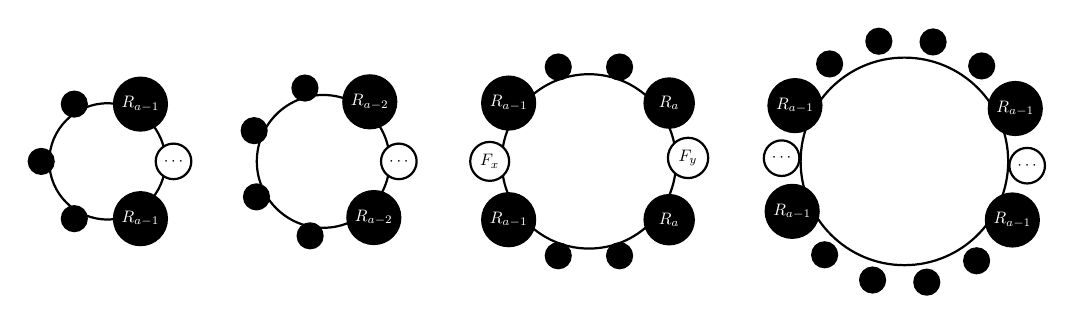
\begin{tikzpicture}[node distance =15em, >=stealth, ->, scale=0.6, transform shape, thick] 

\node[circle, minimum size =7em, draw, thick] (C0){};
\foreach \i in {0, ..., 5} \node[circle, minimum size=1.5em, draw, fill=white, thick]at(\i*60: 1.4) (\i){};

\node[circle, minimum size =1.5em, fill=black, text=white]at(1*60: 1.4) (0){${R_{a-1}}$};
\node[circle, minimum size =1.5em, fill=black]at(2*60: 1.4) (1){};
\node[circle, minimum size =1.5em, fill=black]at(3*60: 1.4) (2){};
\node[circle, minimum size =1.5em, fill=black]at(4*60: 1.4) (3){};
\node[circle, minimum size =1.9em, fill=black, text=white]at(5*60: 1.4) (4){ ${R_{a-1}}$};
\node[circle, draw, minimum size =1.9em, fill=white]at(0*60: 1.4) (5){ $\cdots$};

   
\node[circle, minimum size =8em, draw, thick, right of= C0, node distance = 13em] (C1){};
\foreach \i in {0, ..., 6}
\node[circle, minimum size =1.5em, draw, thick, fill=white, right of= \i, node distance = 13em]at(\i*52: 1.6) (1\i){};

\node[circle, minimum size =1.9em, draw, fill=white, right of=0, node distance = 13em]at(0: 1.6) (10){ $\cdots$};
\node[circle, minimum size =1.5em, fill=black, right of=2, text=white, node distance = 13em]at(1*52: 1.6) (12){ ${R_{a-2}}$};
\node[circle, minimum size =1.5em, fill=black, right of=3, node distance = 13em]at(2*52: 1.6) (13){};
\node[circle, minimum size =1.5em, fill=black, right of=4, node distance = 13em]at(3*52: 1.6) (14){};
\node[circle, minimum size =1.5em, fill=black, right of=5, node distance = 13em]at(4*52: 1.6) (15){};
\node[circle, minimum size =1.5em, fill=black, right of=6, node distance = 13em]at(5*52: 1.6) (16){};
\node[circle, minimum size =1.5em, fill=black, right of=7, text=white, node distance = 13em]at(6*52: 1.6) (17){ ${R_{a-2}}$};

\node[circle, minimum size =10.5em, draw, thick, right of= C1,, node distance = 16em] (C2){};
\foreach \i in {0, ..., 9}
\node[circle, minimum size =1.5em, draw, thick, fill=white, right of= \i, node distance = 29em]at(\i*36: 2.1) (2\i){};

\node[circle, minimum size =1.9em, draw, fill=white, right of=0, node distance = 29em]at(2: 2.1) (20){ $F_y$};
\node[circle, minimum size =3.1em, fill=black, right of=1, text=white, node distance = 29em]at(1*36: 2.1) (22){ ${R_{a}}$};
\node[circle, minimum size =1.5em, fill=black, right of=2, node distance = 29em]at(2*36: 2.1) (23){};
\node[circle, minimum size =1.5em, fill=black, right of=3, node distance = 29em]at(3*36: 2.1) (24){};
\node[circle, minimum size =1.5em, fill=black, right of=4, text=white, node distance = 29em]at(4*36: 2.1) (25){ ${R_{a-1}}$};
\node[circle, minimum size =1.9em, draw, fill=white, right of=5, node distance = 29em]at(5*36: 2.1) (26){ $F_x$};
\node[circle, minimum size =1.5em, fill=black, right of=6, text=white, node distance = 29em]at(6*36: 2.1) (17){ ${R_{a-1}}$};
\node[circle, minimum size =1.5em, fill=black, right of=7, node distance = 29em]at(7*36: 2.1) (18){};
\node[circle, minimum size =1.5em, fill=black, right of=8, node distance = 29em]at(8*36: 2.1) (19){};
\node[circle, minimum size =3.1em, fill=black, right of=9, text=white, node distance = 29em]at(9*36: 2.1) (29){ ${R_{a}}$};


\node[circle, minimum size =12.5em, draw, thick, right of= C0, node distance = 48em] (C3){};
\foreach \i in {0, ..., 13}
\node[circle, minimum size =1.5em, draw, thick, fill=white, right of= \i, node distance = 48em]at(\i*25.5: 2.6) (3\i){};

\node[circle, minimum size =1.9em, draw, fill=white, right of=0, node distance = 48em]at(-2: 2.6) (30){ $\cdots$};
\node[circle, minimum size =1.5em, fill=black, right of=1, node distance = 48em, text=white]at(1*25.5: 2.6) (31){ ${R_{a-1}}$};
\node[circle, minimum size =1.5em, fill=black, right of=2, node distance = 48em]at(2*25.5: 2.6) (32){};
\node[circle, minimum size =1.5em, fill=black, right of=3, node distance = 48em]at(3*25.5: 2.6) (33){};
\node[circle, minimum size =1.5em, fill=black, right of=4, node distance = 48em]at(4*25.5: 2.6) (34){};
\node[circle, minimum size =1.5em, fill=black, right of=5, node distance = 48em]at(5*25.5: 2.6) (35){};
\node[circle, minimum size =1.5em, fill=black, right of=6, node distance = 48em, text=white]at(6*25.5: 2.6) (36){ ${R_{a-1}}$};
\node[circle, minimum size =1.9em, draw, fill=white, right of=7, node distance = 48em]at(7*25.5: 2.6) (37){ $\cdots$};
\node[circle, minimum size =1.5em, fill=black, right of=8, node distance = 48em, text=white]at(8*25.5: 2.6) (31){ ${R_{a-1}}$};
\node[circle, minimum size =1.5em, fill=black, right of=9, node distance = 48em]at(9*25.5: 2.6) (32){};
\node[circle, minimum size =1.5em, fill=black, right of=10, node distance = 48em]at(10*25.5: 2.6) (33){};
\node[circle, minimum size =1.5em, fill=black, right of=11, node distance = 48em]at(11*25.5: 2.6) (34){};
\node[circle, minimum size =1.5em, fill=black, right of=12, node distance = 48em]at(12*25.5: 2.6) (35){};
\node[circle, minimum size =1.5em, fill=black, right of=13, node distance = 48em, text=white]at(13*25.5: 2.6) (36){ ${R_{a-1}}$};
\end{tikzpicture} 
\label{fig:SetUP} 
}

\subfloat[Tower-Completed configurations.]{
\centering
%\includegraphics[scale=1.1]{figtowerComp}
\begin{tikzpicture}[node distance =14em, >=stealth, ->, scale=0.6, transform shape, thick] 

\node[circle, minimum size =7em, draw, thick] (C0){};
\foreach \i in {0, ..., 5}{
\node[circle, minimum size=1.5em, draw, fill=white, thick]at(\i*60: 1.4) (\i){};}

\node[circle, minimum size =1.5em, fill=black, text=white]at(1*60: 1.4) (a0){${R_{a-1}}$};
\node[circle, minimum size =1.5em, fill=black]at(2*60: 1.4) (a1){};
\node[circle, minimum size =1.5em, fill=black]at(4*60: 2) (a3+){};
\node[circle, minimum size =1.5em, fill=black]at(4*60: 1.4) (a3){};
\node[circle, minimum size =1.9em, fill=black, text=white]at(5*60: 1.4) (a4){ ${R_{a-1}}$};
\node[circle, draw, minimum size =1.9em, fill=white]at(0*60: 1.4) (a5){ $\cdots$};
\node[below left = 4em and -1.5em of a4, node distance = 5em] (000) {\large$2a +1 = k$};


   
\node[circle, minimum size = 8em, draw, thick, right of= C0, node distance = 13em] (C1){};
\foreach \i in {0, ..., 6}
\node[circle, minimum size =1.5em, draw, thick, fill=white, right of= \i, node distance = 13em]at(\i*52: 1.6) (1\i){};

\node[circle, minimum size =1.9em, draw, fill=white, right of=0, node distance = 13em]at(0: 1.6) (10){ $\cdots$};
\node[circle, minimum size =1.5em, fill=black, right of=2, text=white, node distance = 13em]at(1*52: 1.6) (12){ ${R_{a-2}}$};
\node[circle, minimum size =1.5em, fill=black, right of=3, node distance = 13em]at(2*52: 1.6) (13){};
\node[circle, minimum size =1.5em, fill=black, right of=4, node distance = 13em]at(2*52: 2.2) (13+){};
\node[circle, minimum size =1.5em, fill=black, right of=5, node distance = 13em]at(5*52: 2.2) (16+){};
\node[circle, minimum size =1.5em, fill=black, right of=6, node distance = 13em]at(5*52: 1.6) (16){};
\node[circle, minimum size =1.5em, fill=black, right of=7, text=white, node distance = 13em]at(6*52: 1.6) (17){ ${R_{a-2}}$};
\node[right of = 000, node distance = 13em](1000) {\large$2a = k$};


\node[circle, minimum size =10.5em, draw, thick, node distance = 16em, right of= C1] (C2){};
\foreach \i in {0, ..., 9}
\node[circle, minimum size =1.5em, draw, thick, fill=white, right of= \i, node distance = 29em]at(\i*36: 2.1) (2\i){};

\node[circle, minimum size =1.9em, draw, fill=white, right of=0, node distance = 29em]at(2: 2.1) (20){ $F_y$};
\node[circle, minimum size =3.1em, fill=black, right of=1, text=white, node distance = 29em]at(1*36: 2.1) (22){ ${R_{a}}$};
\node[circle, minimum size =1.5em, fill=black, right of=2, node distance = 29em]at(3*36: 2.7) (23+){};
\node[circle, minimum size =1.5em, fill=black, right of=3, node distance = 29em]at(3*36: 2.1) (23){};
\node[circle, minimum size =1.5em, fill=black, right of=4, text=white, node distance = 29em]at(4*36: 2.1) (25){ ${R_{a-1}}$};
\node[circle, minimum size =1.9em, draw, fill=white, right of=5, node distance = 29em]at(5*36: 2.1) (26){ $F_x$};
\node[circle, minimum size =1.5em, fill=black, right of=6, text=white, node distance = 29em]at(6*36: 2.1) (17){ ${R_{a-1}}$};
\node[circle, minimum size =1.5em, fill=black, right of=7, node distance = 29em]at(7*36: 2.1) (18){};
\node[circle, minimum size =1.5em, fill=black, right of=8, node distance = 29em]at(7*36: 2.7) (18+){};
\node[circle, minimum size =3.1em, fill=black, right of=9, text=white, node distance = 29em]at(9*36: 2.1) (29){ ${R_{a}}$};
\node[right of = 000, node distance = 29em](2000) {\large$2a +1= k/2 \ \wedge \  y<x$};


\node[circle, minimum size =12.5em, draw, thick, right of= C0, node distance = 48em] (C3){};
\foreach \i in {0, ..., 13}
\node[circle, minimum size =1.5em, draw, thick, fill=white, right of= \i, node distance = 48em]at(\i*25.5: 2.6) (3\i){};

\node[circle, minimum size =1.9em, draw, fill=white, right of=0, node distance = 48em]at(-2: 2.6) (30){ $\cdots$};
\node[circle, minimum size =1.5em, fill=black, right of=1, node distance = 48em, text=white]at(1*25.5: 2.6) (31){ ${R_{a-1}}$};
\node[circle, minimum size =1.5em, fill=black, right of=2, node distance = 48em]at(2*25.5: 2.6) (32){};
\node[circle, minimum size =1.5em, fill=black, right of=3, node distance = 48em]at(2*25.5: 3.2) (32+){};
\node[circle, minimum size =1.5em, fill=black, right of=4, node distance = 48em]at(5*25.5: 3.2) (35+){};
\node[circle, minimum size =1.5em, fill=black, right of=5, node distance = 48em]at(5*25.5: 2.6) (35){};
\node[circle, minimum size =1.5em, fill=black, right of=6, node distance = 48em, text=white]at(6*25.5: 2.6) (36){ ${R_{a-1}}$};
\node[circle, minimum size =1.9em, draw, fill=white, right of=7, node distance = 48em]at(7*25.49: 2.6) (30){ $\cdots$};
\node[circle, minimum size =1.5em, fill=black, right of=8, node distance = 48em, text=white]at(8*25.5: 2.6) (31){ ${R_{a-1}}$};
\node[circle, minimum size =1.5em, fill=black, right of=9, node distance = 48em]at(9*25.5: 2.6) (32){};
\node[circle, minimum size =1.5em, fill=black, right of=10, node distance = 48em]at(9*25.5: 3.2) (32+){};
\node[circle, minimum size =1.5em, fill=black, right of=11, node distance = 48em]at(12*25.5: 3.2) (35+){};
\node[circle, minimum size =1.5em, fill=black, right of=12, node distance = 48em]at(12*25.5: 2.6) (35){};
\node[circle, minimum size =1.5em, fill=black, right of=13, node distance = 48em, text=white]at(13*25.5: 2.6) (36){ ${R_{a-1}}$};
\node[right of = 000, node distance = 48em](3000) {\large$2a +2= k/2$};

\end{tikzpicture}
\label{fig:TowerComp} 
}
\caption{Tower-Creation phase from Set-Up final configurations.} 
\label{fig:TCP} 
\end{figure} 

Informally, for each odd block one tower is formed by the central
robot moving to its neighboring node containing the robot with the
larger view. For each even block two towers are formed by the two
central robots moving to their other neighbors.

The corresponding rules  are described in Table~\ref{tab: rules}, where scheduled
robots stay idle in all cases not covered. The view is given by an $F$-$R$-$T$ sequence
as described in Definition~\ref{def:view}.  Figure~\ref{fig:TCP}
illustrates the process of tower creation from the possible Set-Up
final configurations. Each configuration in Figure~\ref{fig:SetUP}
will produce the one just below in Figure~\ref{fig:TowerComp}. Big
circles contain a set of adjacent nodes which are all free or all
occupied.  A big black node $R_x$ represents $x$ adjacent occupied
nodes, a big white node $F_x$ represents $x$ adjacent free nodes, and
a white node containing dots represents a positive number of free
nodes.

\begin{landscape}
\begin{table*}
\centering
\begin{tabular}{|l l c  l c l|}
\hline
\multicolumn{6}{|l|}{\textbf{Tower-Creation Phase: }} \\[1pt] \hline
Rule:: & Condition & $\land$ & $\view(r, c)$&$\rightarrow$&Move\\
\hline
$TC1_0$:: &{ $2a+1=k$}& $\land$ &${  (R_{a+1}, F_x, R_a)}$&
$\rightarrow$&$r.\?$\\
$TC2_0$:: &{ $2a = k$}&$\land$ &${   (R_{a+1}, F_x, R_{a-1})}$&
$\rightarrow$&$r.\Back$\\
$TC2_1$:: &{ $2a = k$}&$\land$ &${  
 (R_{a}, F_x, R_{a-2}, T_2, F_1)}$&
$\rightarrow$&$r.\Front$\\
$TC3_0$:: &{ $2a+1 = k$, $y<x$}&$\land$ &
${   (R_{a+1}, F_y, R_{k/2}, F_x, R_a)}$&$\rightarrow$&
$r.\Back$\\ 
$TC3_1$:: &{ $2a+1 = k$, $y<x$}&$\land$ &
${   (R_{a+1}, F_y, R_{a}, F_1, T_2, R_{a-1}, F_x, R_a)}$&
$\rightarrow$&$r.\Back$\\
$TC4_0$:: &{ $k/2 = 2a+2$}&$\land$ &
${  (R_{a+2}, F_x, R_{k/2}, F_y, R_{a})}$&
$\rightarrow$&$r.\Back$\\
$TC4_{11}$:: &{ $k/2 = 2a+2$}&$\land$ &
${  (R_{a+1}, F_x, R_{k/2}, F_y, R_{a-1}, T, F_1)}$&
$\rightarrow$&$r.\Front$\\
$TC4_{12}$:: &{ $k/2 = 2a+2$}&$\land$ &
${  (R_{a+2}, F_x, R_{a-1}, F_1, T_2, R_{a-1}, F_y, R_{a})}$&
$\rightarrow$&$r.\Back$\\
$TC4_{13}$:: &{ $k/2 = 2a+2$}&$\land$ &
${  (R_{a+2}, F_x, R_{a-1}, T_2, F_1, R_{a+1}, F_y, R_{a})}$&
$\rightarrow$&$r.\Back$\\ 
$TC4_{21}$:: &{ $k/2 = 2a+2$}&$\land$ &
${  (R_{a+2}, F_x, R_{a-1}, T_2, F_2, T_2, R_{a-1}, F_y, R_{a})}$&
$\rightarrow$&$r.\Back$\\
$TC4_{22}$:: &{ $k/2 = 2a+2$}&$\land$ &
${  (R_{a+1}, F_x, R_{a+1}, F_1, T, R_{a-1}, F_y, R_{a-1}, T, F_1)}$&
$\rightarrow$&$r.\Front$\\
$TC4_{23}$:: &{ $k/2 = 2a+2$}&$\land$ &
${  (R_{a+1}, F_x, R_{a-1}, T, F_1, R_{a+1}, F_y, R_{a-1}, T, F_1)}$&
$\rightarrow$&$r.\Front$\\
$TC4_{3}$:: &{ $k/2 = 2a+2$}&$\land$ &
${  (R_{a+1}, F_x, R_{a-1}, T, F_2, T, R_{a-1}, F_y, R_{a-1} T, F_1)}$&
$\rightarrow$&$r.\Front$\\ \hline 
\multicolumn{6}{l}{ } \\[1pt] \hline
\multicolumn{6}{|l|}{\textbf{Exploration Phase: }} \\[1pt] \hline
Rule:: & Condition & $\land$ & \multicolumn{1}{l}{$\view(r, c)$}&$\rightarrow$&Move\\
\hline
$E_1$:: &{$2a+1=k, \ x \geq 1$}&$\land$&
\multicolumn{1}{l}{${   (R_1, F_x, R_a, F_1, T_2, R_{a-2}, F_y)}$}&
$\rightarrow$& $r.\Front$\\
%&&&&\\
$E_2$:: &{$2a = k$, $x > 0$,  $z < (n-k+2)/2$ }&$\land$&
\multicolumn{1}{l}{${ 
(R_1, F_x, R_1, F_y, R_{a-3}, T_2, F_2, T_2, R_{a-3}, F_z)}$}&
$\rightarrow$& $r.\Front$\\
%  $z < (x+y+z)/2$ and $y < (x+y+z)/2$}\\
%A vérifier 
%&&&&\\
%pas tour
$E_{31}$:: &$2a+1 = k/2 $, $g< (g+b+c)/2$&$\land$&
\multicolumn{1}{l}{${   
(R_1, F_b, R_1, F_c, R_{a-2}, T_2, F_1, R_{a-1}, F_d, }$}&&\\
		&&&\multicolumn{1}{r}{
${  R_1, F_e, R_1, F_f, R_{a-1}, F_1, T_2, R_{a-2}, F_g)}$}&
$\rightarrow$&$r.\Front$\\

%tour
$E_{32}$:: &$2a+1 = k/2 $, $d < (d+e+f)/2$&$\land$&
\multicolumn{1}{l}{${   
(R_1, F_e, R_1, F_f, R_{a-1}, F_1, T_2, R_{a-2}, F_g, R_1, }$}&&\\
                 &&&\multicolumn{1}{r}{
${ F_b, R_1, F_c, R_{a-2}, T_2,  F_1, R_{a-1}, F_d)}$}&
$\rightarrow$&$r.\Front$\\
%&&&&\\
$E_{4}$:: 	&{$2a+2 = k/2 $,  $g< (g+b+c)/2$}&$\land$&
\multicolumn{1}{l}{${   
(R_1, F_{b}, R_1, F_{c}, R_{a-2}, T_2, F_2, T_2, R_{a-2}, F_d, }$}&&\\
		&&&\multicolumn{1}{r}{
${  R_1, F_{e}, R_1, F_f, R_{a-2}, T_2, F_2, T_2, R_{a-2}, F_{g})}$}&
$\rightarrow$&$r.\Front$\\
\hline
\end{tabular}
\caption{Rules of the Tower-Creation and Exploration phases  for a robot $r$.}
\label{tab: rules}
\end{table*}
\end{landscape}

There are four cases: 
\begin{itemize}
\item If there is only one block of odd size then the Set-Up final
  configuration looks like the first one of Figure~\ref{fig:SetUP}. A
  unique robot can move according to rule $TC1_0$, which produces the
  configuration just below in Figure~\ref{fig:TowerComp} (or the
  symmetric one with the tower in the upper half instead of the
  lower half).
\item If there is only one block of even size (second column), then
  two robots will move according to rule $TC2_0$. If one has moved
  before the other one could take a snapshot of the configuration then
  its movement is given by rule $TC2_1$.
\item If there are two symmetric blocks of odd size (third case), 
  then two robots will move according to rule $TC3_0$. If one has moved
  before the other one could take a snapshot of the configuration then
  its movement is obtained by rule $TC3_1$. In this case, the two free
  segments $F_x$ and $F_y$ have different sizes, and the robots move
  in the direction opposite to the shortest one.
\item If there are two blocks of even size (rightmost column) then
  robots move according to rule $TC4_0$. In this case also, the two
  free segments have different sizes.  If one tower is formed, the
  other robot movement is given by rules $TC4_{11}$, $TC4_{12}$ and
  $TC4_{13}$ according to the robot view.  If two of them have moved, 
  and two towers are formed, then the moving robots compute their
  movements according to one of the rules in $\{TC4_{21}, TC4_{22}, 
  TC4_{23}\}$, depending of which robots have moved before.  And when
  all robots but one have moved, the last one moves according to rule
  $TC4_3$.
\end{itemize}

\subsection{The Exploration Phase} \label{exp}
The exploration phase is the last phase of the algorithm. It starts
from tower-completed configurations and is described in the second part of
Table~\ref{tab: rules} (where again robots stay idle for non covered
cases). No new towers are created during this phase.


Note that the empty nodes adjacent to towers have already been
explored, so the segments of empty nodes between the blocks are the
only ones possibly not yet explored. Each of these segments is
explored in the current phase by one or two robots closest to the
segment.


When $k$ is odd, the configuration starting the exploration phase is
made of two blocks, one of them containing a tower (leftmost
configuration of Figure~\ref{fig:TowerComp}).  The explorer is the
robot at the border of the block with the tower, the tower being the
other border of the block. Its destination is the
neighbor free node toward the block that does not contain the tower.
The algorithm for the moving robot is given by rule $E_1$.

When $k$ is even, there are as many explorers as blocks from the
tower-completed configuration.  An explorer is a robot at a border of
a block, and which is adjacent to an empty segment not visited. Their
destinations are their adjacent node towards the center of the empty
segment.  The explorers keep being isolated robots until they either
are neighbors in the middle of the segment (when the empty segment is
even) or they form another tower (when the empty segment has odd
size).  The corresponding rules of the algorithm are: $E_2$, $E_{31}$, 
$E_{32}$ and $E_4$.


		%%
		\section{Results: Bounds refined}
Using model-checking tools on this
formal representation of the algorithm, we show that it satisfies the
exploration and termination properties under fairness hypothesis (see
Section \ref{subsub: specification}) in the asynchronous model.  Hence, the algorithm is correct
for all tested instances of $k$ and $n$ that satisfy the constraints
given in the original paper: $n$, $k$ are co-prime and $n, k \geq 17$.
 
\begin{table}[h]
\centering
{ \centering \begin{tabular}{|c|c|r|r|}
\hline \textbf{k} & \textbf{n} & \textbf{Time} &\textbf{Mem (kB)} \\ \hline 
17 & 18 & 00: 00: 04 & 60\, 984 \\ \hline
18 & 19 & 00: 00: 04 & 66\, 256 \\ \hline 
17 & 19 & 00: 25: 29 & 1\, 622\, 180 \\ \hline 
19 & 20 & 00: 00: 08 & 88\, 168 \\ \hline 
18 & 20 & 00: 12: 10 &2\, 130\, 824 \\ \hline 
17& 20  & 08: 08: 00 & 22\, 045\, 016 \\ \hline 
20 & 21 & 00: 00: 08 & 100\, 136 \\\hline 
19 & 21 & 01: 08: 12 & 3\, 632\, 488 \\ \hline
18 & 21 & 03: 00: 52 & 9\, 427\, 620 \\ \hline 
17 & 21 & 18: 40: 07 &55\, 287\, 000 \\ \hline 
21 & 22 & 00: 00: 12 & 123\, 920 \\ \hline 
20 & 22 &01: 58: 27 & 5\, 913\, 880 \\ \hline 
19 & 22 & 08: 25: 22 & 30\, 243\, 392 \\ \hline
18 & 22 & 20: 32: 45 & 100\, 327\, 682 \\ 
\hline 
\end{tabular}}
\caption{Set-Up phase model-checking.} 
\label{tab: flo2}
\end{table}
\begin{table}[htbp] 
\centering
{  
\begin{tabular}{|c|c|r|r|r|}
%{|n|k|States|Transitions|Memory|} 
\hline 
\textbf{k} & \textbf{n} & \textbf{States} & \textbf{Transitions} & 
\textbf{Mem (kB)}  \\ \hline 
5 & 6 & 147 & 436 & 163\, 600 \\ \hline 
5 & 7 & 500 & 1\, 410 & 171\, 084  \\ \hline 
5 & 8 & 2\, 786 & 10\, 596 & 183\, 840  \\ \hline 
5 & 9 & 5\, 533 & 18\, 746 & 207\, 788  \\ \hline 
5 & 10 & 5\, 123\, 204 & 25\, 755\, 007 & 668\, 396 \\ \hline 
5 & 11 & 7\, 827 & 23\, 898 & 299\, 980  \\ \hline 
5 & 12 & 13\, 996 & 61\, 822 & 380\, 244  \\ \hline 
5 & 13 & 17\, 149 & 82\, 902 & 491\, 708  \\ \hline 
5 & 14 & 30\, 680 & 157\, 829 & 637\, 840 \\ \hline 
5 & 15 & 19\, 784\, 312 & 130\, 057\, 237 & 2\, 667\, 850 \\ \hline 
5 & 16 & 12\, 418 & 73\, 688 & 1\, 081\, 736  \\ \hline 
5 & 17 & 33\, 004 & 207\, 642 & 1\, 401\, 280  \\ \hline 
5 & 18 & 10165 & 66\, 120 & 1\, 790\, 644  \\ \hline 
\hline 
7 & 8 & 680 & 1860 & 171\, 396 \\ \hline 
7 & 9 & 2\, 764 & 7\, 576 & 201\, 096 \\ \hline 
7 & 10 & 3\, 022 & 9\, 220 & 270\, 676 \\ \hline 
7 & 11 & 16\, 471 & 56\, 390 & 437\, 876 \\ \hline 
7 & 12 & 18\, 347 & 42\, 448 & 754\, 680 \\ \hline 
7 & 13 & 20\, 272 & 83\, 706 & 1\, 352\, 120 \\ \hline
\hline 
10 & 11 & 839 & 1942 & 190\, 884  \\ \hline 
10 & 12 & 3\, 834 & 8\, 868 & 460\, 750  \\ \hline 
10 & 13 & 7\, 924 & 23\, 731 & 756\, 000  \\ \hline 
10 & 14 & 8\, 357 & 27\, 524 & 2\, 135\, 987  \\ \hline 
\end{tabular}}
\caption{Model-checking small instances of the entire algorithm.} 
\label{tab: flo+}
\end{table}

Since the most complex phase of the algorithm is the Set-Up phase, we
present in Table~\ref{tab: flo2} the verification results (time and
memory) for the restriction to this particular phase, model-checking
the property: every run reaches a configuration satisfying the Type$D$
predicate (corresponding to a Set-Up final configuration).  The state
space explosion occurring during the model-checking can be seen on
these results.

We also tested the algorithm for some small instances not covered by
the original setting. Interestingly, our methodology permits to refine
the correctness bounds for these cases. The performances can be seen
in Table~\ref{tab: flo+}, where the algorithm satisfies the correctness
property for all values of $n$ and $k$ appearing in the table. 

From these experiments, we conjecture that the algorithm is correct
for $n\leq 18$ in the following cases even when $n$ and $k$ are not
co-prime, as long as the initial configuration is not periodic (where
not periodic means that there is at most one symmetry axis in the
ring and that it is not invariant by non-trivial rotation): 
\begin{itemize}%[parsep=0cm, itemsep=0cm, topsep=0cm]
\item When $k$ is even the algorithm is correct as long as $n <
  k+\lceil k/2 \rceil$ and $10\leq k < 17$.
\item When $k$ is odd the algorithm is correct if $5\leq k < 17$.
\end{itemize}
Unfortunately, the combinatorial explosion made the verification
exceed reasonable time for some cases. For instance, the computation
was stopped for $k=7$ and $n=14$ after $1$ day.

We outline here the number of states and the number of transitions in
order to show that the memory and the time used increase as the number
of transitions and states of the system.  Moreover, when $k$ and $n$
are not co-prime these numbers explode, due to the complexity of
the algorithm to ensure the exploration when there are symmetries.


We now recall the problem of perpetual exclusive
ring exploration, and present the verification results for the
\emph{Min-Algorithm}~\cite{blin_exclusive_2010}.



%%%%%%%%%%%%%%%%%%%%%%%%%%%%%%%%%%%%%%%%%%%%%%%%%%%%%%%%%
%%%%%%%%%%%%%%%%%%%%%%%%%%%    MIN    %%%%%%%%%%%%%%%%%%%%%%%%%
%%%%%%%%%%%%%%%%%%%%%%%%%%%%%%%%%%%%%%%%%%%%%%%%%%%%%%%%%
	\chapter{\emph{Min-Algorithm}}
	\label{sec:min}
We first remark that the same arguments as in~\cite{flocchini_computing_2007} 
apply to obtain impossibility when the number $k$ of robots divides 
the size $n$ of the ring. 
For this algorithm, model checking tools are used to exhibit a
counter-example.  After identifying the rule producing this
counter-example, we correct the algorithm and establish the
correctness of the new version by model checking small instances and
providing an inductive proof.

	\section{Specification of the perpetual exploration without collision}
	\label{subsub:perpexp} 
For any ring and any initial configuration
where each node is occupied by at most one robot, an algorithm solves
the perpetual exclusive exploration problem if it guarantees the
following two properties: 
\begin{itemize}%[parsep=0cm, itemsep=0cm, topsep=0cm]
\item[\emph{(i)}] \emph{Exclusivity}: There is at most one robot on
  any vertex and two robots never  cross the same edge at the same
  time in opposite directions.
\item[\emph{(ii)}] \emph{Liveness}: Each robot visits each node 
infinitely often.
\end{itemize}
These properties can be expressed in \textsf{LTL} (see Section~\ref{def:LTL}) as follows: the
\emph{Exclusivity} property is the conjunction of the
\emph{No\_collision} and the \emph{No\_switch} properties below: 
\begin{itemize}%[parsep=0cm, itemsep=0cm, topsep=0cm] 
\item
 \emph{No\_collision}: ~$\G\Big(\bigwedge\limits_{1\leq j<h}^k c(r_j) \neq c(r_{h})\Big)$
\item
  \emph{No\_switch}: ~$\bigwedge\limits_{i=1}^n\bigwedge\limits_{\substack{j=1}}^k
\bigwedge\limits_{\substack{h=1}}^k\neg~\Diamond
  \Big(c(r_j)=i~\wedge~c(r_h)=i+1~\wedge~r_j.\Front~\wedge~r_{h}.
\Back\Big)$
\end{itemize}
The \emph{No\_collision} property states that there is always at most
one robot on each node, while the \emph{No\_switch} property states
that two neighbor robots cannot exchange their position by moving in
opposite directions along an edge: one of them moves $\Front$
while the other moves $\Back$.  Note that the
\emph{No\_collision} property implies the \emph{No\_switch} property
in the asynchronous model, since one of the possible executions that
form a tower is obtained when two neighbors want to switch their
positions, and their moves are executed asynchronously.

In order to express that each robot visits all vertices infinitely
often, we use the \emph{Live} property: 

$$\textit{Live}: ~\bigwedge\limits_{i=1}^n\bigwedge\limits_{j=1}^k
\G\F\big(c(r_j)=i\big).$$

The \textit{Liveness} property needs the fairness assumption. Hence, it
can be expressed by: 

$$\textit{Liveness}: \textit{Fairness} \Rightarrow \textit{Live}.$$

		%%
		\section{The algorithm}
	\label{subsec:mindef}
The \emph{Min-Algorithm} from~\cite{blin_exclusive_2010} is designed
to ensure that $3$ robots always exclusively and perpetually explore
any ring of size $n \geq 10$ where $n$ is not a multiple of $3$.  It
is based on a classification of the set of tower-free configurations.
The \emph{Min-Algorithm} operates in two phases: the
\emph{Convergence} phase and the \emph{Legitimate} phase.  In the
\emph{Convergence} phase system states converge towards so-called
\emph{Legitimate states}. In the \emph{Legitimate} phase the system
cycles between its legitimate states, performing the exploration.  

In Definitions~\ref{def:L} and~\ref{def:NL} below, each set of
configurations is an equivalence class of configurations, given by an
$F$-$R$-$T$ sequence, according to Definition~\ref{def:view}.

\begin{definition}
  \label{def:L}\emph{Legitimate configurations} are defined for $n\geq
  10$ by $\mathbb{L}^n = L1^n \cup L2^n \cup L3^n$ where: 
\begin{itemize}%[parsep=0cm, itemsep=0cm, topsep=0cm] 
\item$L1^n=(R_2, F_2, R_1, F_{n-5} )$
\item $L2^n=(R_1, F_1, R_1, F_{n-6}, R_1, F_2)$
\item $L3^n=(R_1, F_3, R_2, F_{n-6})$
\end{itemize}
\end{definition}

All other (tower free) configurations are called \emph{non legitimate
  configurations}. We denote by $\mathbb{NL}^n$ the set of non
legitimate configurations and we also partition $\mathbb{NL}^n$
according to the number of consecutive robots. This leads to the five
sets $A^n$, $B^n$, $C^n$, $D^n$, $ E^n$ defined below.

\begin{definition}
  \label{def:NL} \emph{Non legitimate configurations} are defined for
  $n\geq 10$, when $n$ and $3$ are co-prime, by $\mathbb{NL}^n = A^n \cup B^n \cup C^n \cup D^n \cup
  E^n$ as follows.\\ When one robot is at the same distance of the two
  others, wether there are robots on two neighbor nodes or not, then it is a $B^n$ configuration: 
  $$\begin{array}{ll}B^n = &\{(R_1, F_x, R_1, F_y, R_1, F_x) \mid \ 
x > 0 \ \wedge \ x\neq y  \wedge \ n = 2x+y+3\}. \end{array}$$
  Otherwise: 
\begin{itemize}%[parsep=0cm]
\item If no robots are neighbors, it is a $C^n$ configuration: 
 $$\noindent C^n=\{(R_1, F_x, R_1, F_y, R_1, F_z) \mid  \ 
   0< x<z<y \wedge \ (x, z) \neq (1, 2)\wedge \ n=x+y+z+3\}$$
 Note that the case $(x, z)=(1, 2)$ corresponds to a $L2^n$ configuration. 
 Hence, $C^n$ configurations only appear when $n\geq 11$.
\item If only two robots are neighbors, if the minimal distance
  between these two robots and the last one is equal to $2$ or $3$, 
  then it is a $L1^n$ or a $L3^n$ configuration. Otherwise: 
		\begin{itemize}
		\item If the minimal distance is equal to $1$, then it
                  is an $E^n$ configuration: \\ $E^n=(R_1, F_1, R_2, 
                  F_{n-4}).$
		\item Otherwise the distance is larger than $3$ and
                  then it is an $A^n$ configuration: 
 $\begin{array}{ll}A^n=&\{(R_1, F_x,  R_2, F_z) 
   \mid 4 \leq x < z \wedge \ n = x+z+3\}. 
\end{array}$\\
 Note that this type of configuration only exists when $n>12$, since
 $n$ and $k=3$ must be co-prime.
		\end{itemize}
	\item If the three robots are neighbors
		then the configuration is a $D^n$ configuration: \\
		$D^n=(R_3, F_{n-3}).$
\end{itemize}
\end{definition}

From the disjunction of cases in Definitions~\ref{def:L} and
\ref{def:NL} above, and observing that no two sets of
configurations overlap, we have: 
\begin{proposition}\label{prop: partition}
  The sets of configurations: $A^n$, $B^n$, $C^n$, $D^n$, $E^n$, 
  $L1^n$, $L2^n$, $L3^n$, form a partition of the set of all
  tower-free configurations of a ring of size $n \geq 10$, when $n$
  and $k=3$ are co-prime.
\end{proposition}

\begin{table*}[tbp]
\small{
\centering
\begin{tabular}{|l l c l c l|}
%{|n|k|States|Transitions|Memory|Model|Verif|}
\hline
\multicolumn{6}{|l|}{ \rule[0.1cm]{0cm}{0.25cm} 
\textbf{Legitimate Phase: }} \\[1pt] \hline
Rule:: & Condition & $\land$ & \multicolumn{1}{l}{$\view(r, c)$}&$\rightarrow$&Move\\
\hline
$RL1$:: &&&$(R_2, F_2, R_1, F_{n-5})$& $\rightarrow$&$r.\Back$\\
$RL2$:: &&&$(R_1, F_1, R_1, F_{n-6}, R_1, F_2)$&$\rightarrow$&$r.\Front$\\
$RL3$:: &&&$(R_1, F_3, R_2, F_{n-6})$&$\rightarrow$&$r.\Front$\\
\hline
\multicolumn{5}{l}{ } \\[1pt] \hline
\multicolumn{6}{|l|}{\rule[0.1cm]{0cm}{0.25cm}  
\textbf{Convergence Phase: }}
\\ \hline
Rule:: & Condition & $\land$ & \multicolumn{1}{l}{$\view(r, c)$}&$\rightarrow$&Move\\
\hline
$RC1$:: &$4 \leq x < z$&$\wedge $&$(R_1, F_x, R_2, F_z)$&$\rightarrow$&$r.\Front$\\
$RC2$:: &$x \neq y$, $x > 0$ &$\wedge $&
$(R_1, F_x, R_1, F_y, R_1, F_x)$&$\rightarrow$&$r.\?$\\
$RC3$:: &$0<x<z<y \wedge (x, z) \neq (1, 2)$&$\wedge $&
$(R_1, F_x, R_1, F_y, R_1, F_z)$&$\rightarrow$&$r.\Front$\\
$RC4$:: &&&$(R_3, F_{n-3})$&
$\rightarrow$&$r.\Back$\\
$RC5$:: &&&$(R_1, F_1, R_2, F_{n-4})$&
$\rightarrow$&$r.\Back$\\
\hline
\end{tabular}}
\caption{Rules of \emph{Min-Algorithm}~\cite{blin_exclusive_2010} 
for a robot $r$ with $n \geq 10$.}
\label{tab: algo-min}
\end{table*}

\medskip We now detail the two phases, described in Table~\ref{tab: algo-min}.
In the \emph{Legitimate} phase the idea is to authorize, by exploiting
the asymmetry of the network, a single robot to move at each step.
Rule $RL1$ authorizes only the robot which is the farthest from the
isolated robot to move.  This robot goes to the only free neighboring
node.  Rule $RL2$ authorizes the robot which is the nearest to the
other robots to move in order to minimize the distance between him and
his nearest neighbor.  Rule $RL3$ authorizes the isolated robot to
come closer to the other robots.  After the execution of $n$ rounds
(each one of the three robots has moved $n$ times), all robots have
explored the ring once.
  
The \emph{Convergence} phase 
brings non-legitimate configurations into legitimate ones. The main
point of this algorithm is to break possible symmetries and to
converge to a pattern that allows the execution of one of the $RL$
rules.  Rule $RC1$ (resp. $RC2$, $RC3$, $RC4$ and $RC5$) is only
applied for configurations in $A^n$ (resp. $B^n$, $C^n$, $D^n$, 
$E^n$). Rule $RC1$ is applied in order to reduce the distance between
the isolated robot and the two other robots. Rule $RC2$ is applied
when a robot is at equal distance from the two other robots.  This
robot will break the symmetry by a shift of one position in any
direction. Rule $RC3$ is applied when robots are scattered on the ring
at distances $x<z<y$. The robot authorized to move is the one that is
adjacent to the free spaces of size $x$ and $z$. This robot will move
such that the free space $x$ is reduced by $1$. The idea behind this
movement is to create a block of robots. Rule $RC4$ captures the
situation when the three robots are neighbors.  In this case, due to
the symmetry the two robots on the border can move.
Rule $RC5$ is applied when the isolated robot is too close (at
distance $1$) to the block of robots. In this case it will move away
from the block.


The specification for this algorithm is refined as follows: 
\begin{itemize}%[parsep=0cm, itemsep=0cm, topsep=0cm]
\item[\emph{(a)}] The \emph{No\_collision} and \emph{No\_switch}
  properties are satisfied.
\item[\emph{(b)}]  From any non-legitimate configuration a
  legitimate configuration is reached.
\item[\emph{(c)}] The exploration is performed by cycling within the
  legitimate configurations (ensuring the \emph{Liveness} property).
\end{itemize}

		%
		\section{Results: A counter example}
		
Recall that the setting of the \emph{Min-Algorithm} features $3$
robots in a ring of size $n \geq 10$ where $n$ is not a multiple of
$3$. Thus, we first construct a model for this protocol and its
properties in the model checker DiVinE~\cite{Divine13}. Then
we verify this algorithm for the smallest possible ring (of size $10$) 
for all models (Fsync, Ssync and Async). These results are presented
in Table~\ref{tab: min}, with number of states, transitions, and memory
used.
 
\begin{table}[htbp] 
\centering
\setlength{\tabcolsep}{4pt}
\begin{tabular}{|r|r|r|c|c|} 
%{|n|k|States|Transitions|Memory|Model|Verif|}
\hline 
\textbf{States} & \textbf{Transitions} & \textbf{Mem(kB)}&
\textbf{Model} & \textbf{Result} \\ 
\hline 256\, 315 & 737\, 810 &~~248\, 668 & ~Fsync~ & ok \\ 
\hline 407\, 175 & 881\, 437 & 248\, 840 & Ssync &ok\\ 
\hline 3\, 429\, 715 & 13\, 218\, 742 & 1\, 269\, 432 & Async & col \\
\hline 
\end{tabular}
\caption{Model-checking of \emph{Min-Algorithm} in the
3 models for the smallest ring.} 
\label{tab: min} 
\end{table}

More importantly, our results show that the algorithm does not satisfy
the \emph{Exclusivity} property in the Async model. A counter-example
is automatically generated, exhibiting a sequence of transitions
leading to a collision (a tower), Hence, a violation of the
\emph{Exclusivity} property. It is presented in details in Figure
\ref{fig:CE}, with a sequence of configurations obtained by successive
robot moves. In each configuration a computation is represented by an
arrow, which is dotted when the computation is made from an outdated
snapshot.

\begin{figure*}[htbp] 
\centering
\subfloat{
\centering
\includegraphics{figures/figCE1}
\label{fig:CE1} 
}\\\vspace{-2em}
\subfloat{
\centering
\includegraphics{figures/figCE2}
\label{fig:CE2} 
}
\caption{Counter-example.} 
\label{fig:CE} 
\end{figure*} 
 
In the starting configuration after the \textit{LC} phase of all
robots, the gray one and the black one have decided to move according
to the $RC4$ rule, and the light gray one to stay idle.  The black
robot moves, which produces the second configuration. Before the gray
robot could move, the black one performs its \textit{LC} phase and
according to the $RC5$ rules, it chooses to roll away from the two
other robots. The gray robot moves from the decision taken previously
and the third configuration is reached.  From this configuration the
light gray robot performs its \textit{LC} phase and chooses to move in
any direction (as the configuration has an axis of symmetry passing through
this robot). The scheduler makes it move toward the gray one.  From
the fourth configuration thus obtained, the gray robot had to move
according to rule $RL1$ after its \textit{LC} phase.  This movement
permits to obtain the fifth configuration, from where the light gray
robot chooses to move according to rule $RL2$.  We obtain the sixth
configuration thanks to the movement of the black robot (movement that
he had chosen in the second configuration).  From this configuration
the black robot chooses to move according to rule $RC4$, and the move
is performed.  In the last configuration the gray robot performs its
\textit{LC} phase and according to the $RL2$ rule, it chooses to move
toward the light gray one, on the same node where the light gray one
had chosen to go in the fifth configuration.  From there if these two
robots move, they collide.

In this counter-example, we can see that the collision is due to a sequence 
of movements made from outdated snapshots. Hence, we need to stop these 
movements.  We now
present a correction of the algorithm referred to as
\emph{Min-Algorithm-Corrected}. The change concerns the convergence
phase, the legitimate phase being unchanged.  More precisely, only
rule $RC5$ is modified to avoid collisions induced by the previous
rules, when movements computed on obsolete observations are taken into
account. The new $RC5$ rule is: 
$$RC5~~:: ~~(R_2, F_1, R_1, F_{n-4})~~\rightarrow~~r.\Back$$

Note that the moving robot has changed with respect to the old rule.
If this new rule is applied in the counter-example, then from the second
configuration, no movements from outdated snapshots can be made any
more since the $RC5$ rule requires a configuration where the light
gray and the black robots have stayed idle.

\begin{table}[!h] 
\centering 
\setlength{\tabcolsep}{5pt}
\begin{tabular}{|c|r|r|r|c|r|}
%{|n|k|States|Transitions|Memory|Model|Verif|Itérations|} 
\hline \textbf{n} &
\textbf{States} & \textbf{Transitions} & \textbf{Mem(kB)}&
\textbf{Time} \\ \hline 
10& ~1\, 581\, 961 & 6\, 090\, 209 & ~1\, 416\, 880 & 00: 06: 45 \\ \hline 
11& 1\, 926\, 385 & 7\, 421\, 315 & 1\, 568\, 748 & 00: 09: 09 \\ \hline 
13&2\, 716\, 637 & 10\, 476\, 317 & 2\, 252\, 600 & 00: 20: 46 \\ \hline 
14& 3\, 162\, 409 &12\, 307\, 905 & 2\, 560\, 724 & 00: 26: 54 \\ \hline 
16& 4\, 155\, 385 & 16\, 041\, 365& 2\, 772\, 188 & 00: 36: 22 \\ \hline 
\end{tabular} \caption{Model-checking of the
\emph{Min-Algorithm-Corrected}.} \label{tab: correct} \end{table}

Verification results (where correctness is obtained) are given in
Table~\ref{tab: correct} for several instances of $n$. All results
show a limited blow up, due to the fact that when the number $k=3$ of
robots is fixed, the maximal number of configurations (and of states) is
of order $n^3$.




		
		
		
		